\documentclass{book}
\usepackage{amsmath}
\usepackage{graphicx}
\usepackage{hyperref}
\usepackage{amssymb}
\usepackage{amsfonts}
\usepackage{tcolorbox}
\usepackage{hyperref}
\usepackage[latin1]{inputenc}
\graphicspath{ {./images/} }

\hypersetup{
    colorlinks=true,
    linkcolor=cyan,
    filecolor=magenta,      
    urlcolor=blue,
}

\title{Calculus Single Variable}
\author{Robert Ghrist}
\date{11/15/16}

\newbox\bwk\edef\tempd#1pt{#1\string p\string t}\tempd\def\nbextr#1pt{#1}
\def\npts#1{\expandafter\nbextr\the#1\space}
\def\ttwplink#1#2{\special{ps:1 0 0 setrgbcolor}#2\special{ps:0 0 0 setrgbcolor}\setbox\bwk=\hbox{#2}\special{ps:( linkto #1)\space\npts{\wd\bwk} \npts{\dp\bwk} -\npts{\ht\bwk} true\space Cpos}}
\begin{document}
\boldmath
\maketitle

\tableofcontents{}

\begin{sloppypar}
\part{Calculus Single Variable}

\chapter{Functions} \label{ChFunctions}

\section{Functions} \label{ChFunctionsSecFunctions}

A \textit{function} can be visualized as a machine that takes in an input $x$ and returns an output $f(x)$. The collection of all possible inputs is called the \textit{domain}, and the collection of all possible outputs is called the \textit{range}.\\
This course deals with functions whose domains and ranges are $\mathbb{R}$ or subsets of $\mathbb{R}$ (this is the notation for the real numbers).\\\\
\textbf{Examples}
\begin{enumerate}
\item Polynomials, e.g. ${f(x) = x^3-5x^2+x+9}$. Give the domain and range of $f$.\\
Answer: The domain is $\mathbb{R}$, because we can plug in any real number into a polynomial. The range is $\mathbb{R}$, which we see by noting that this is a cubic function, so as ${x \rightarrow -\infty}$, ${f(x) \rightarrow -\infty}$, and as ${x \rightarrow \infty}$, ${f(x) \rightarrow \infty}$.
\item Trigonometric functions, e.g. $\sin$, $\cos$, $\tan$. Give the domain and range for each of these.\\
Answer: For $\sin$ and $\cos$: domain is $\mathbb{R}$; range is ${\left[-1,1\right]}$. For $\tan$, the domain is ${\lbrace x \in \mathbb{R}: x \neq \frac{\pi}{2}+k\pi\rbrace}$; range is $\mathbb{R}$.
\item The exponential function, $e^x$. Give the domain and range for the exponential.\\
Answer: Domain is $\mathbb{R}$; range is (${(0,\infty)}$.
\item The natural logarithm function, ${\ln x}$. Recall that this is the inverse of the exponential function. Give the domain and range for ${\ln x}$.\\
Answer: Domain is $(0,\infty)$; range is $\mathbb{R}$. Notice how the domain and range of the exponential relate to the domain and range of the natural logarithm.
\item Is ${\sin^{-1}}$ a function? If so, why? If not, is there a way to make it into a function?
\\Answer: ${\sin^{-1}}$ is not a function, because one input has many outputs. For example, ${\sin^{-1}(0) = 0,\pi,2\pi,\ldots}$. By restricting the range of ${\sin^{-1}}$ to ${\displaystyle\left[-\frac{\pi}{2},\frac{\pi}{2}\right]}$, one gets the function $\arcsin$.
\end{enumerate}

\subsection{Operations on Functions} \label{ChFunctionsSubsOperationsOnFunctions}

\textbf{Composition}\\
The \textit{composition} of two functions, $f$ and $g$, is defined to be the function that takes as its input x and returns as its output $g(x)$ fed into $f$.
\begin{equation*} f\circ g(x)=f(g(x)) \end{equation*}
\\
\textbf{Example:}\\
${\sqrt{1-x^{2}}}$ can be thought of as the composition of two functions, $f$ and $g$. If ${g=1-x^{2}}$, $f$ would be the function that takes an input $g(x)$ and returns its square root.\\\\
\textbf{Example:}\\
Compute the composition ${f \circ f}$, i.e. the composition of $f$ with itself, where ${\displaystyle f(x) = \frac{1}{x+1}}$.\\
Answer:\\
We find that
\begin{align*}
f \circ f(x)&=f(f(x))\\
&=f \left(\frac{1}{x+1}\right)\\
&=\frac{1}{1/\left(x+1\right)+1}\\
&=\frac{x+1}{1+x+1}\\
&=\frac{x+1}{x+2}.
\end{align*}
\\\\
\textbf{Inverse}\\
The \textit{inverse} is the function that undoes $f$. If you plug ${f(x)}$ into ${f^{-1}}$, you will get $x$. Notice that this function works both ways. If you plug ${f^{-1}(x)}$ into $f(x)$, you will get back $x$ again.
\begin{equation*} f^{-1}(f(x))=x \end{equation*} 
\begin{equation*} f(f^{-1}(x))=x \end{equation*}
NOTE: ${f^{-1}}$ denotes the inverse, not the reciprocal. ${f^{-1}(x)\neq\frac{1}{f(x)}}$.\\\\
\textbf{Example:}\\
Let's consider ${f(x)=x^{3}}$. Its inverse is ${f^{-1}(x)=x^{\frac{1}{3}}}$.
\begin{equation*} f^{-1}(f(x))=(x^{3})^{\frac{1}{3}}=x \end{equation*}
\begin{equation*} f(f^{-1}(x))=(x^{\frac{1}{3}})^{3}=x \end{equation*}
Notice that the graphs of $f$ and $f^{-1}$ are always going to be symmetric about the line ${y=x}$. That is the line where the input and the output are the same.

\subsection{Classes of Functions} \label{ChFunctionsSubsClassesOfFunctions}

\textbf{Polynomials}\\
A polynomial $P(x)$ is a function of the form 
\begin{equation*} P(x)=c_{0}+c_{1}x+c_{2}x^{2}+\dots+c_{n}x^{n} \end{equation*}
The top power $n$ is called the degree of the polynomial. We can also write a polynomial using a summation notation.
\begin{equation*} P(x)=\sum_{k=0}^{n}c_{k}x^{k} \end{equation*}\\
\textbf{Rational functions}\\
Rational functions are functions of the form ${\displaystyle\frac{P(x)}{Q(x)}}$ where each is a polynomial.\\\\
\textbf{Example:}\\
\begin{equation*} \displaystyle\frac{3x-1}{x^{2}+x-6} \end{equation*} is a rational function. You have to be careful of the denominator. When the denominator takes a value of zero, the function may not be well-defined.\\\\
\textbf{Powers}\\
Power functions are functions of the form ${cx^{n}}$, where $c$ and $n$ are constant real numbers.\\
Other powers besides those of positive integers are useful.\\\\
\textbf{Example:}\\
What is ${x^{0}}$ ?\\
Answer:\\
${x^{0}=1}$\\\\
What is ${x^{-\frac{1}{2}}}$ ?\\
Answer:\\
Recall a fractional power denotes root. For example, ${x^{\frac{1}{2}}=\sqrt{x}}$. The negative sign in the exponent means that we take the reciprocal. So, ${x^{-\frac{1}{2}}=\frac{1}{\sqrt{x}}}$.\\\\
What is ${x^\frac{22}{7}}$ ?\\
Answer:\\
One can rewrite this as ${\left(x^{22}\right)^{1/7}}$. That means we take $x$ to the 22nd power and then take the 7th root of the result.\\
${x^\frac{22}{7}=\sqrt[7]{x^{22}}}$\\\\
What is ${x^{\pi}}$ ? We are not yet equipped to handle this, but we will come back to it later.\\\\
\textbf{Trigonometrics}\\
You should be familiar with the basic trigonometric functions $\sin$, $\cos$. One fact to keep in mind is ${\cos^{2} \theta +\sin^{2} \theta=1}$ for any $\theta$. This is known as a \textit{Pythagorean identity}, which is so named because of one of the ways to prove it:
\begin{center}
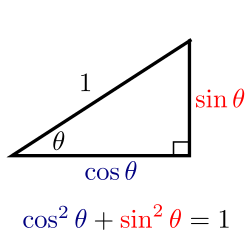
\includegraphics[scale=0.5]{Pythagorean}
\end{center}
By looking at a right triangle with hypotenuse 1 and angle $\theta$, and labeling the adjacent and opposite sides accordingly, one finds by using Pythagoras' Theorem that ${\cos^2 \theta + \sin^2 \theta = 1}$.\\
Another way to think about it is to embed the above triangle into a diagram for the unit circle where we see that ${\cos\theta}$ and ${\sin\theta}$ returns the x and y coordinates, respectively, of a point on the unit circle with angle $\theta$ to the $x$-axis:
\begin{center}
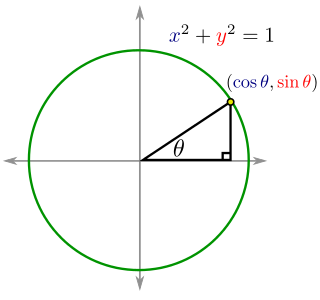
\includegraphics[scale=0.5]{UnitCircle}
\end{center}
That explains the nature of the formula ${\cos^{2} \theta+\sin^{2} \theta=1}$. It comes from the equation of the unit circle ${x^2 + y^2 = 1}$.\\
Others trigonometric functions:\\
${\tan=\displaystyle\frac{\sin}{\cos}}$\\
${\cot=\displaystyle\frac{\cos}{\sin}}$ , the reciprocal of $\tan$\\
${\sec=\displaystyle\frac{1}{\cos}}$ , the reciprocal of the $\cos$\\
${\csc=\displaystyle\frac{1}{\sin}}$ , the reciprocal of the $\sin$\\\\
All four of these have vertical asymptotes at the points where the denominator goes to zero.\\\\
\textbf{Inverse Trigonometrics}\\
We often write ${\sin^{-1}}$ to denote the inverse, but this can cause confusion. Be careful that ${\sin^{-1}\neq\displaystyle\frac{1}{\sin}}$. To avoid the confusion, the terminology $\arcsin$ is recommended for the inverse of the $\sin$ function.\\
The $\arcsin$ function takes on values ${\left[-\displaystyle\frac{\pi}{2},\frac{\pi}{2}\right]}$ and has a restricted domain ${\left[-1,1\right]}$.\\
The $\arccos$ function likewise has a restricted domain ${\left[-1,1\right]}$, but it takes values ${\left[0,\pi\right]}$.\\
The $\arctan$ function has an unbounded domain, it is well defined for all inputs. But it has a restricted range ${\displaystyle\left(-\frac{\pi}{2},\frac{\pi}{2}\right)}$.\\\\
\textbf{Exponentials}\\
Exponential functions are of the form ${c^x}$, where $c$ is some positive constant. The most common such function, referred to as \textit{the} exponential, is ${e^x}$. This is the most common because of its nice integral and differential properties (below).\\
Algebraic properties of the exponential function:\\
\begin{equation*} \displaystyle e^{x}e^{y}=e^{x+y} \end{equation*}
\begin{equation*} \displaystyle (e^{x})^{y}=e^{xy} \end{equation*}
Differential/integral properties:\\
\begin{equation*} \displaystyle\frac{d}{dx} e^{x}=e^{x} \end{equation*}
\begin{equation*} \displaystyle\int e^{x}dx=e^{x}+C \end{equation*}
Recall the graph of ${e^x}$, plotted here alongside its inverse, ${\ln x}$:\\
\begin{center}
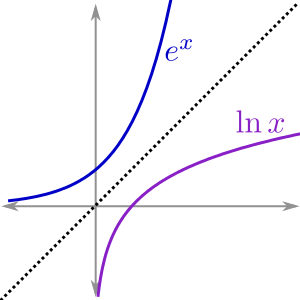
\includegraphics[scale=0.5]{ExpLn}
\end{center}
Note that the graphs are symmetric about the line ${y = x}$ (as is true of the graphs of a function and its inverse).\\
Before continuing, one might ask, what is $e$? There are several ways to define $e$, which will be revealed soon. For now, it is an irrational number which is approximately 2.718281828.\\\\
\textbf{Euler's Formula}\\
To close this lesson, we give a wonderful formula, which for now we will just take as a fact:\\
\begin{tcolorbox}
Euler's Formula
\begin{equation*} e^{ix}=\cos x+i\sin x \end{equation*}
\end{tcolorbox}
The $i$ in the exponent is the imaginary number ${\sqrt{-1}}$. It has the properties ${i^{2}=-1}$. $i$ is not a real number. That doesn't mean that it doesn't exist. It just means it is not on a real number line.\\
Euler's formula concerns the exponentiation of an imaginary variable. What exactly does that mean? How is this related to trigonometric functions? This will be covered in our next lesson.\\\\
\textbf{Additional Examples}\\\\
\textbf{Example:}\\
Find the domain of \[ f(x) = \frac{1}{\sqrt{x^2 -3x+2}}. \]
Answer:\\
te that the square root is only defined when its input is non-negative. Also, the denominator in a rational function cannot be 0. So we find that this function is well-defined if and only if ${x^2-3x+2>0}$. Factoring gives \[ (x-2)(x-1) > 0. \]
By plotting the points ${x=1}$ and ${x=2}$ (where the denominator equals 0) and testing points between them, one finds that ${x^2-3x+2>0}$ when ${x<1}$ or ${x>2}$:
\begin{center}
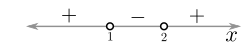
\includegraphics[scale=0.5]{PointChecking}
\end{center}
So the domain of $f$ is ${x<1}$ or ${2<x}$. In interval notation, this is ${\left(-\infty,1\right) \cup \left(2, \infty \right)}$.\\\\
\textbf{Example:}\\
Find the domain of \[ f(x) = \ln(x^3-6x^2+8x). \]
Answer:\\
Since $\ln$ is only defined on the positive real numbers, we must have ${x^3-6x^2+8x>0}$. Factoring gives \[ x(x^2-6x+8) = x(x-2)(x-4)>0 \]
As in the above example, plotting the points where this equals 0 and then testing points, we find that the domain is ${0<x<2}$ and ${4<x}$. In interval notation, this is ${\left(0,2 \right) \cup \left(4,\infty\right)}$.

\section{The Exponential} \label{ChFunctionsSecTheExponential}

This module deals with a very important function: the exponential. The first question one might ask is: what is the exponential function ${e^x}$? We know certain values of the function such as ${e^0=1}$, but what about an irrational input such as ${e^\pi}$, or an imaginary input ${e^i}$? Is it possible to make sense of these values?\\
The following definition answers these questions.\\
\begin{tcolorbox}
The Exponential $e^x$
\begin{align*} 
e^x &= 1+x+\frac{x^2}{2!} + \frac{x^3}{3!} + \frac{x^4}{4!} + \dotsb 
& = \sum_{k=0}^\infty \frac{x^k}{k!}, 
\end{align*}
where \[ k! = k(k-1)(k-2)\dotsb 3 \cdot 2 \cdot 1, \] and ${0! = 1}$
\end{tcolorbox}
One can now plug values for $x$ into the above sum to compute ${e^x}$. When ${x=0}$, for instance, one finds that ${e^0=1}$, (since all the terms with $x$ disappear) as expected. By plugging in ${x=1}$, the true value of $e$ is found to be ${e=1+1+\frac{1}{2!}+\frac{1}{3!}+\dotsb}$.\\\\
\textbf{A long polynomial}\\
There are technical concerns when trying to add up an infinite number of things. These issues will be dealt with later in the modules on \ref{ChDiscretizationSecSeries}{series}. For now, treat the infinite sum above as a long polynomial (the actual term is the Taylor series about ${x=0}$, which will be more formally dealt with in the next module). Polynomials are nice because they are easy to integrate and differentiate. Recall the power rule for differentiating and integrating a monomial ${x^k}$, where $k$ is a constant:
\begin{align*}
\frac{d}{dx} x^k &= kx^{k-1} 
\int x^k \, dx &= \frac{1}{k+1} x^{k+1} + C \quad (k \neq -1) 
\end{align*}
\\\textbf{Properties of $e^x$}\\
Recall the following properties of the exponential function:
\begin{enumerate}
\item ${e^{x+y} = e^xe^y}$
\item ${e^{x\cdot y}=(e^x)^y=(e^y)^x}$
\item ${\frac{d}{dx}e^x = e^x}$
\item ${\int e^x dx=e^x+C}$.
\end{enumerate}
Consider the last two properties in terms of the long polynomial.Taking the derivative of the long polynomial for ${e^x}$ gives
\begin{align*} 
\frac{d}{dx}(1+x+\frac{x^2}{2!}+\frac{x^3}{3!} + \frac{x^4}{4!} + \dotsb)
&= 0 + 1 + \frac{2x}{2!} + \frac{3x^2}{3!} + \frac{4 x^3}{4!} + \dotsb\\
&= 1 + x + \frac{x^2}{2!} + \frac{x^3}{3!} + \dotsb,
\end{align*}
which is the original long polynomial. Integrating also gives (up to the constant of integration) the original long polynomial. This agrees with facts about the derivative and integral of ${e^x}$. Thus, the long polynomial for ${e^x}$ captures two of the key features of ${e^x}$; namely, ${e^x}$ is its own derivative and its own integral.\\\\
\textbf{Euler's formula}\\
Recall that the imaginary number $i$ is defined by ${i=\sqrt{-1}}$. So ${i^2=-1}$, ${i^3=-i}$, ${i^4=1}$, and this continues cyclically (for a review of complex/imaginary numbers, see \href{https://en.wikipedia.org/wiki/Complex_number}{wikipedia}). Assume the following fact, known as Euler's formula, mentioned in the last module.
\begin{tcolorbox}
	Euler's formula
	\begin{equation*} e^{ix} = \cos x + i \sin x. \end{equation*}
\end{tcolorbox}
Consider what happens when $ix$ is plugged into the long polynomial for ${e^x}$. By simplifying the powers of $i$, and grouping the result into its real and imaginary parts, one finds
\begin{align*} 
e^{ix} &= 1+ix+\frac{(ix)^2}{2!}+\frac{(ix)^3}{3!} + \dotsb\\
&= 1 + ix + \frac{i^2 x^2}{2!} + \frac{i^3 x^3}{3!} + \dotsb\\
&= 1 + ix - \frac{x^2}{2!} - i\frac{x^3}{3!} + \frac{x^4}{4!} + i \frac{x^5}{5!} + \dotsb\\
&= \left(1 - \frac{x^2}{2!} + \frac{x^4}{4!} - \dotsb\right) + i \left(x - \frac{x^3}{3!} + \frac{x^5}{5!} - \dotsb \right).
\end{align*}

\section{Taylor series} \label{ChFunctionsSecTaylorSeries}
\section{Computing Taylor series} \label{ChFunctionsSecComputingTaylorSeries}
\section{Convergence} \label{ChFunctionsSecConvergence}
\section{Expansion points} \label{ChFunctionsSecExpansionPoints}
\section{Limits} \label{ChFunctionsSecLimits}
\section{L'Hopital's Rule} \label{ChFunctionsSecLHopitalsRule}
\section{Orders of growth} \label{ChFunctionsSecOrdersOfGrowth}

\chapter{Differentiation} \label{ChDifferentiation}
\section{Derivatives} \label{ChDifferentiationSecDerivatives}
\section{Differentiation rules} \label{ChDifferentiationSecDifferentiationRules}
\section{Linearization} \label{ChDifferentiationSecLinearization}
\section{Higher derivatives} \label{ChDifferentiationSecHigherDerivatives}
\section{Optimization} \label{ChDifferentiationSecOptimization}
\section{Differentials} \label{ChDifferentiationSecDifferentials}
\section{Differentiation as an operator} \label{ChDifferentiationSecDifferentiationAsAnOperator}

\chapter{Integration} \label{ChIntegration}
\section{Antidifferentiation} \label{ChIntegrationSecAntidifferentiation}
\section{Exponential growth examples} \label{ChIntegrationSecExponentialGrowthExamples}
\section{More differential equations} \label{ChIntegrationSecMoreDifferentialEquations}
\section{ODE Linearization} \label{ChIntegrationSecODELinearization}
\section{Integration by Substitution} \label{ChIntegrationSecIntegrationBySubstitution}
\section{Integration by parts} \label{ChIntegrationSecIntegrationByParts}
\section{Trigonometric substitution} \label{ChIntegrationSecTrigonometricSubstitution}
\section{Partial fractions} \label{ChIntegrationSecPartialFractions}
\section{Definite integrals} \label{ChIntegrationSecDefiniteIntegrals}
\section{Fundamental Theorem of Integral Calculus} \label{ChIntegrationSecFundamentalTheoremOfIntegralCalculus}
\section{Improper integrals} \label{ChIntegrationSecImproperIntegrals}
\section{Trigonometric integrals} \label{ChIntegrationSecTrigonometricIntegrals}
\section{Tables and computers} \label{ChIntegrationSecTablesAndComputers}

\chapter{Applications} \label{ChApplications}

\chapter{Discretization} \label{ChDiscretization}
\section{Series} \label{ChDiscretizationSecSeries}

\end{sloppypar}
\end{document}
